\usetikzlibrary{bayesnet}
\scalebox{0.7}{
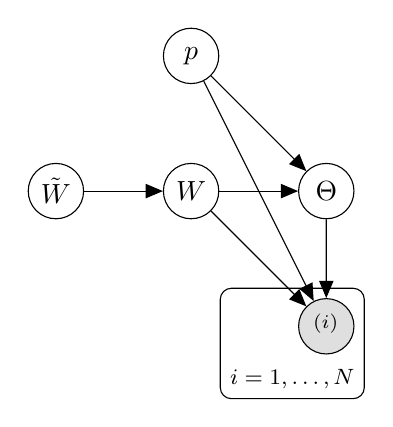
\begin{tikzpicture}[scale=3]

  % Define nodes
  \node[latent] (Wtilde) {$\tilde{W}$};
  \node[latent, right=of Wtilde] (W) {$W$};
  \node[latent, above=of W] (p) {$p$};
  \node[latent, right=of W] (Theta) {$\Theta$};
  \node[obs, below=of Theta] (x) {$\vx^{(i)}$};
  
  % Connect nodes
  \edge {Wtilde} {W};
  \edge {p} {x};
  \edge {W} {Theta};
  \edge {W} {x};
  \edge {Theta} {x};
  \edge {p} {Theta};
  
  % Define plate
  \plate {x_plate} {(x)} {$i = 1, \dots, N$};

\end{tikzpicture}
}